\documentclass[a4paper]{article}
\usepackage[affil-it]{authblk}

\usepackage[margin=1in]{geometry}
\setlength{\parskip}{3pt}
\usepackage{hyperref}
\usepackage{mathrsfs}
\usepackage{tikz}
\usetikzlibrary{shapes}

\usepackage{clrscode}

\begin{document}
    \title{One-Way Quantum Communication Complexity}
    \author{Dominic Moylett\thanks{\texttt{\href{dominic.moylett@bristol.ac.uk}{dominic.moylett@bristol.ac.uk}}}}
    \affil{Quantum Engineering Centre for Doctoral Training,\\University of Bristol}
    \date{\today}
    \maketitle

    \begin{abstract}
        Communication complexity is the study of how much information two or more parties need to share with each other in order to perform joint computation of a problem. There are many benefits to this model of computation, from many lower bound proofs to applications in cryptography and data streaming. In this report, we will summarise the most exciting recent trends in the one-way form of quantum communication complexity, look at what quantum speedups already exist and what problems are still open.
    \end{abstract}

    \section{Introduction}

    \section{Communication Complexity}

        Communication complexity was developed by Yao in 1979 as an analysis of distributed computing \cite{Yao:1979:CQR:800135.804414}. Under this model of computation, our computation is done between two parties, commonly referred to as Alice and Bob, with inputs $x, y \in \{0, 1\}^n$, respectively. The two parties do not know each other's inputs; Alice does not know $y$ and Bob does not know $x$. Alice and Bob then exchange a series of messages between each other through a protocol established before computation, with their aim being to jointly compute $f(x, y)$. The question communication complexity asks is how many bits of information do Alice and Bob need to communicate in order for the two of them to compute a solution. We offer a sketch of a typical communication complexity problem in Figure~\ref{fig:cc}.

        A na\"{i}ve solution to any communication complexity problem can be completed using $n$ bits of communication: Alice sends $x$ to Bob and Bob then does all of the computation for $f(x, y)$. So the question then becomes if it is possible to compute $f(x, y)$ with $o(n)$ bits of communication.

        \begin{figure}
            \centering
            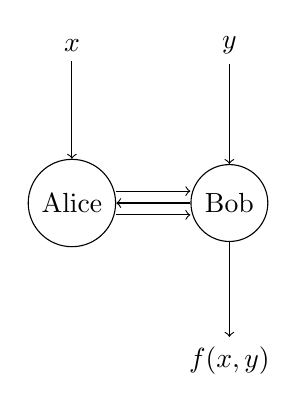
\begin{tikzpicture}[->, draw, node distance=2cm]
                \node[circle, draw] (Alice) at (0,0) {Alice};
                \node[circle, draw] (Bob) [right of=Alice] {Bob};
                \node (x) [above of=Alice] {$x$};
                \node (y) [above of=Bob] {$y$};
                \node (bout) [below of=Bob] {$f(x, y)$};
                \path
                    (x) edge (Alice)
                    (y) edge (Bob)
                    (Bob) edge (bout);
                \path ([yshift=1ex]Alice.east) edge ([yshift=1ex]Bob.west);
                \path (Bob.west) edge (Alice.east);
                \path ([yshift=-1ex]Alice.east) edge ([yshift=-1ex]Bob.west);
            \end{tikzpicture}
            \caption{An example of communication complexity. Alice and Bob begin computation with bit strings $x$ and $y$. They then exchange a series of messages based on a pre-determined protocol. Computation completes when Bob outputs $f(x, y)$.}
            \label{fig:cc}
        \end{figure}

        In quantum communication complexity, first proposed in 1993 by Yao \cite{366852}, we also have parties Alice and Bob given inputs $x$ and $y$, respectively, and have to produce $f(x, y)$ for some function $f$. But now our two parties can send quantum messages between each other, and the complexity is measured in the number of qubits that are communicated.

        Another model by Burhman and Cleve \cite{quant-ph/9704026} does not use the physical sending of data between the parties, but instead uses the measurement of entangled particles for remote computation. Our focus for this report however will be on the former. Note that it is possible to simulate this model by the ability to communicate quantum states: Alice generates entangled pairs of qubits and sends one of the pair to Bob. Likewise, it is possible to simulate communicating $l$ qubits by use of $l$ entangled pairs and $2l$ classical bits of communication, via quantum teleportation \cite{PhysRevLett.70.1895}.

        \subsection{One-Way Communication Complexity}

        A specific subset of communication complexity, which we will focus on throughout this report, is one-way communication complexity. In this model of computation, Alice and Bob again receive respective inputs $x, y \in \{0, 1\}^n$ with the aim of Bob being able to output $f(x, y)$ for some function $f$. The difference now is that only one message is allowed to be sent, from Alice to Bob. This is illustrated in \ref{fig:ow-cc}.

        Like general communication complexity, one-way communication complexity can also be solved na\"{i}vely in $n$ bits of communication by Alice sending $x$ to Bob. So once again, our question is if we can do better with less communication.

        \begin{figure}
            \centering
            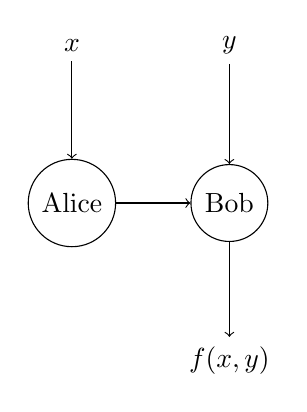
\begin{tikzpicture}[->, draw, node distance=2cm]
                \node[circle, draw] (Alice) at (0,0) {Alice};
                \node[circle, draw] (Bob) [right of=Alice] {Bob};
                \node (x) [above of=Alice] {$x$};
                \node (y) [above of=Bob] {$y$};
                \node (bout) [below of=Bob] {$f(x, y)$};
                \path
                    (x) edge (Alice)
                    (y) edge (Bob)
                    (Bob) edge (bout);
                \path (Alice.east) edge (Bob.west);
            \end{tikzpicture}
            \caption{An example of one-way communication complexity. Alice receives input $x$ and Bob receives input $y$. Alice then sends a single message to Bob. Using this additional information from Alice, Bob performs and outputs the computation $f(x, y)$.}
            \label{fig:ow-cc}
        \end{figure}

        \subsection{Holevo's Theorem}

        Even before Yao's work on the formalisation of Communication Complexity, it was clear that quantum communication would not be able to speed up some problems. In particular, a consequence of Holevo's theorem \cite{Hol73}, meant that while a message of $n$ bits could be compressed into a message of at most $n-1$ qubits, the same message could not be retrieved from said qubits. We phrase this as a one-way communication complexity problem below.

        \begin{codebox}
            \Procname{Problem $\proc{COMMUNICATION}$}
            \zi \const{Alice's input:} $x \in \{0, 1\}^n$.
            \zi \const{Bob's input:} none.
            \zi \const{Bob's output:} $x$.
        \end{codebox}

    By Holevo's theorem, we know that the above problem requires Alice to send $\Omega(n)$ qubits to Bob. A later proof by Nayak \cite{814608} shows that if we compress a message of $n$ bits into a message of $m < n$ qubits, the probability that we can successfully retrieve all $n$ bits again is at most $2^{m-n}$. The only exception to this is when Alice and Bob have shared entangled qubits between each other prior to computation, in which case superdense coding can be used to send two bits by sending one qubit \cite{PhysRevLett.69.2881}. Brassard \cite{quant-ph/0101005} explains that if we have unlimited entanglement between Alice and Bob then we can only at most reduce the amount of communication by a factor of $1/2$, as quantum teleportation can be used to send qubits from one party to the other using entangled pairs and communicating with classical bits \cite{PhysRevLett.70.1895}.

    While we cannot do communication of $n$ bits with fewer than $n$ qubits, we will in the next two sections look at more specific problems which we can solve by communication of fewer qubits.

    \section{Functions}

        \subsection{Distributed Deutsch-Jozsa}

        The Distributed Deutsch-Jozsa problem, first introduced by Buhrman, Cleve and Wigderson \cite{Buhrman:1998:QVC:276698.276713}, was the first example of an exponential separation between quantum and classical computation complexity. The problem, and its quantum protocol as described in Buhrman et al.~\cite{RevModPhys.82.665}, are stated as follows, where $\mathcal{D}(x, y)$ is the Hamming distance between $x$ and $y$ and $U_x = \sum_{i=0}^{n-1}(-1)^{x_i}|i\rangle\langle i|$ for $x \in {0, 1}^n$:

        \begin{codebox}
            \Procname{Protocol $\proc{DISTRIBUTED DEUTSCH-JOZSA}$}
            \zi \const{Alice's input:} $x \in \{0, 1\}^n$.
            \zi \const{Bob's input:} $y \in \{0, 1\}^n$.
            \zi \const{Promise:} $x = y$ or $\mathcal{D}(x, y) = n/2$.
            \zi \const{Bob's output:} $0$ iff $x = y$, $1$ otherwise.
            \li Alice starts computation in the $|0\rangle^{\otimes \log n}$ state and applies $U_xH^{\otimes \log n}$ to get the state $|\psi\rangle$.
            \li Alice sends $|\psi\rangle$ to Bob.
            \li Bob applies $H^{\otimes \log n}U_y$ and measures in the computational basis.
            \li Bob outputs $0$ if they measure $|0\rangle^{\otimes \log n}$ and 1 otherwise.
            \End
        \end{codebox}

        The state Alice sends to Bob is $|\psi\rangle = \frac{1}{\sqrt{n}}\sum_{i=0}^{n-1} (-1)^{x_i}|i\rangle$. When Bob applies $U_y$ to this state, they end up with the state $\frac{1}{\sqrt{n}}\sum_{i=0}^{n-1}(-1)^{x_i}(-1)^{y_i}|i\rangle$. We'll now consider this state for two situations: one where $x = y$ and one where they differ in $n/2$ places, denoted $|\psi_0\rangle$ and $|\psi_1\rangle$, respectively.

        Note that if $x = y$ then $(-1)^{x_i}(-1)^{y_i} = 1$, so $|\psi_0\rangle = \frac{1}{\sqrt{n}}\sum_{i = 0}^{n-1}|i\rangle$. $|\psi_1\rangle$ on the other hand will have exactly $n/2$ amplitudes which are positive, and $n/2$ amplitudes which are negative. From this we can see that $\langle\psi_0|\psi_1\rangle = \frac{n/2 - n/2}{n} = 0$, so the states can be distinguished from one another upon measurement. Finally, Bob's application of $H^{\otimes \log n}$ converts their state to the computational basis. Note that $H|\psi_o\rangle = |0\rangle^{\otimes\log n}$, so measuring this state will indicate that $x = y$ and any other state will indicate that $\mathcal{D}(x, y) = n/2$.

        So we have been able to deterministically solve this problem with $O(\log n)$ qubits of communication between Alice and Bob. How much classical communication is required to solve it? It was shown in Appendix 4 of Buhrman et al.~\cite{RevModPhys.82.665} that any deterministic protocol must send at least $0.007n$ bits from Alice to Bob, otherwise the protocol will fail for some input. However, this quantum advantage is lost when compared to randomised classical computation for some positive integer $c$:

        \begin{codebox}
            \Procname{Protocol $\proc{DISTRIBUTED DEUTSCH-JOZSA}$}
            \li Alice picks $c$ unique items $a \in \{0, 1\}^n$ uniformly at random.
            \li Alice sends $(a_i, x_{a_i})~ \forall i \in \{0,...,c-1\}$.
            \li Bob returns $0$ if $x_{a_i} = y_{a_i}~ \forall i \in \{0,...,c-1\}$, and $1$ otherwise.
            \End
        \end{codebox}

        Bob always returns $0$ if $x = y$, so our protocol has no true negative results. If $\mathcal{D}(x, y) = n/2$, then the protocol fails if $x_{a_i} = y_{a_i} \forall i \in \{0,...,c-1\}$, which happens with probability $1/2^c$. Finally, note that each $a_i$ can be communicated in $\log n$ bits, so the overall communication required is $c(\log n + 1)$ bits.

        \subsection{Subgroup Membership}

        We saw one disadvantage of the Distributed Deutsch-Jozsa problem above was that a quantum protocol has no advantage over a randomised classical protocol. Another disadvantage is that the problem requires a {\em promise} on the input: that either the two bit strings are identical or they differ in exactly $n/2$ places. This promise results in a very contrived problem with little practical application. This begs the question: Are there any problems which do not rely on promises that yield a quantum advantage under the communication complexity model?

        While this is still an open problem in quantum communication complexity, there are some problems which have shown potential. Aaronson et al.~\cite{0902.3175} were the first to explore the problem of subgroup membership as potentially yielding a quantum advantage. Their protocol for solving subgroup membership, based on an earlier quantum algorithm by Watrous \cite{Watrous:2000:SQP:795666.796590}, is described below, where $G$ is a group, $\mathscr{H}_G$ is the set of all subgroups of $G$, $|+\rangle = \frac{1}{\sqrt{2}}(|0\rangle + |1\rangle)$ and $U_{G, y} = \sum_{g \in G}|yg\rangle\langle g|$ for some $y \in G$:

        \begin{codebox}
            \Procname{Protocol $\proc{SUBGROUP-MEMBERSHIP}$}
            \zi \const{Alice's input}: $H \in \mathscr{H}_G$.
            \zi \const{Bob's input}: $y \in G$.
            \zi \const{Bob's output}: $1$ if $y \in H$, $0$ otherwise.
            \li Alice prepares the state $|H\rangle = \frac{1}{\sqrt{|H|}}\sum_{h \in H}|h\rangle$, which is then sent to Bob.
            \li Bob prepends an ancilla qubit to get $|H\rangle|+\rangle$ and applies $U_{G, y}$ controlled on the final qubit.
            \li Bob applies a Hadamard to the second qubit and measures in the computational basis.
        \end{codebox}

        Any element $h \in H$ can be described in $\lceil\log |G|\rceil$ bits, so Alice needs to send $O(\log |G|)$ qubits to Bob in order to perform this protocol.

        After line 2, Bob has the state $\frac{1}{\sqrt{2}}(|H\rangle|0\rangle + |yH\rangle|1\rangle)$, where $|yH\rangle = \frac{1}{\sqrt{|H|}}\sum_{yh \in H}|h\rangle$. If $y \in H$ then $yh \in H~ \forall h \in H$, so $|yH\rangle = |H\rangle$. Therefore, if $y \in H$ then $U_{G, y}|H\rangle|+\rangle = |H\rangle|+\rangle$, so applying a Hadamard to the final qubit makes the final qubit $|0\rangle$. A measurement in the computational basis will thus always yield $0$.

        On the other hand, if $y \notin H$ then $\langle yH|H\rangle = 0$, so applying the Hadamard produces

        $$\frac{1}{2}(|H\rangle|0\rangle + |H\rangle|1\rangle + |yH\rangle|0\rangle - |yH\rangle|1\rangle).$$

        Measuring the final qubit will result in $|0\rangle$ -- and thus a false positive -- with probability $1/2$. We can repeat this protocol a constant number of times to get a negligible error probability.

        \subsection{Permutation Invariance}

    \section{Relations}

        \subsection{Hidden Matching}

        \subsection{$\alpha$-matching}

    \section{Applications}

    \section{Implementations}

    \section{Conclusion}

        \subsection{Open Problems}

        \subsection{Other Areas}

    \bibliographystyle{plain}
    \bibliography{quantum_communication_complexity}{}
\end{document}